\documentclass[12pt, a4paper, twoside, openany]{book}
\usepackage[
    a4paper, 
    total={6in, 8in}, 
    top=2cm,
    left=3cm,
    right=2.5cm,
    bottom=1.25cm,
    includeheadfoot,
    headheight=40pt,
]{geometry}
\usepackage[T1]{polski}
\usepackage{graphicx}
\usepackage{fancyhdr}
\usepackage{mathptmx}
\usepackage{enumitem}
\usepackage[utf8]{inputenc}
\usepackage{import}
\usepackage{setspace}
\usepackage{titlesec}
\usepackage{multirow}
\usepackage{longtable}

\import{../}{commands.tex}

\fancypagestyle{plain}{
    \fancyhf{}
    \renewcommand{\headrulewidth}{0pt}
    \fancyhead[C]{\uniimage}
    \fancyfoot[LE,RO]{\thepage}
}

% Wymogi edycyjne: https://moodle2.e-wsb.pl/pluginfile.php/7505508/mod_resource/content/2/Wymogi%20edycyjne_praca%20dyplomowa.pdf

\renewcommand\thesection{\Alph{chapter}\arabic{section}}

\linespread{1.5}

\setlist[itemize]{label=--}

\begin{document}

% Header & footer settings :)
\pagestyle{plain}

\titleformat
{\chapter} %/{〈command 〉}
[block] %/[〈shape〉]
{\bfseries\large} %/ {〈format〉}
{} %/ {〈label 〉}
{0.5ex} %/ {〈sep〉}
{
    \centering
} %/ {〈before-code〉}
{
    \vspace{-0.5ex}%
} %/ {〈after-code〉}

\setcounter{secnumdepth}{4}

\titleformat{\section}[hang]{\normalfont\bfseries}{\thesection.}{0.5em}{}

\titleformat{\subsection}[hang]{\normalfont\bfseries}{\thesubsection.}{0.4em}{}

\titleformat{\subsubsection}[hang]{\normalfont\bfseries}{\thesubsubsection.}{0.4em}{}

\begin{titlepage}
    \begin{center}

        \uniimage

        \MakeUppercase{\department}

        \vspace{5cm}

        \begin{Large} \textbf{\topic} \end{Large}

        \vspace{5cm}

        PROJEKT DYPLOMOWY

        \vfill
        Poznań 2023

    \end{center}
\end{titlepage}

\setcounter{tocdepth}{3}
\tableofcontents

\chapter{\MakeUppercase{dane partnerów}}

\section{Dane Promotora}

\begin{tabular}{ |p{5cm}|p{7cm}|}
    \hline
    Imię i nazwisko         & Izabela Janicka-Lipska \\
    \hline
    Stopień / Tytuł naukowy & dr. inż.               \\
    \hline
    Data i podpis           &                        \\ \hline
\end{tabular}

\section{Dane członków Zespołu projektu}

\membersTable


% Example table and figure formatting
\section{Wprowadzenie}
Lorem ipsum dolor sit amet, consectetur adipiscing elit. Fusce nec justo eu urna accumsan tincidunt. Aliquam erat volutpat.

\chapter{\MakeUppercase{Założenia projektu}}

\section{Opis Projektu}

\subsection{Uzasadnienie wyboru tematu}

Problem utylizacji odpadów stał się w ostatnich latach jednym z największych wyzwań dla społeczeństwa i środowiska naturalnego. Śmieci są produkowane w ogromnych ilościach, a nieprawidłowe postępowanie z nimi prowadzi do skażenia powietrza, wody i gleby. W związku z tym, istnieje potrzeba opracowania rozwiązań, które ułatwią zarządzanie odpadami w sposób bardziej skuteczny i zrównoważony.

Dzięki rozwojowi technologii uczenia maszynowego, pojawiła się możliwość stworzenia aplikacji mobilnej, która rozpoznawać będzie pojemniki na odpady na podstawie zdjęć oraz oznaczać je na mapie. Ułatwi ona lokalizowanie pojemników na dany typ odpadów oraz proces właściwego utylizowania śmieci dla użytkowników. Taka aplikacja może również zwiększyć świadomość społeczną w zakresie utylizacji odpadów i przyczynić się do zmniejszenia ilości odpadów zalegających na składowiskach.


Temat ten jest aktualny i ważny, a jednocześnie daje wiele możliwości na zastosowanie różnych technologii i algorytmów uczenia maszynowego. Przy realizacji projektu można wykorzystać m.in. sieci neuronowe, algorytmy uczenia głębokiego, przetwarzanie obrazów, uczenie maszynowe w chmurze oraz usługi geolokalizacyjne.

Podsumowując, projekt \topic jest uzasadniony ze względu na aktualność i ważność tematu, możliwość wykorzystania najnowszych technologii oraz potencjalne korzyści dla społeczeństwa i środowiska naturalnego.

\subsection{Problem badawczy}

Problemem badawczym jest określenie algorytmów uczenia maszynowego najlepiej nadających się do rozpoznawania pojemników na odpady na podstawie zdjęć oraz określenie cech obrazów odpowiadających za skuteczność modelu.

W ramach tego problemu badawczego można skoncentrować się na kilku podproblemach, m.in.:
\begin{itemize}
    \item analiza dostępnych zbiorów danych:
          \begin{itemize}
              \item znalezienie zbiorów danych do treningu i testowania modelu rozpoznawania pojemników na odpady;
              \item określenie jak są one zdefiniowane oraz jakie informacje zawierają.
          \end{itemize}
    \item wybór odpowiednich algorytmów uczenia maszynowego:
          \begin{itemize}
              \item określenie algorytmów uczenia maszynowego, które najlepiej nadają się do rozpoznawania pojemników na odpady na podstawie zdjęć.
          \end{itemize}
    \item przygotowanie zbiorów danych:
          \begin{itemize}
              \item zastosowanie technik przetwarzania obrazów;
              \item potencjalne użycie technik augmentacji danych.
          \end{itemize}
    \item implementacja i trening modelu: wyłonienie najlepszej techniki trenowania modelu bazowanego na obrazach;
    \item ocena skuteczności modelu: określenie metryk, które pozwolą dokładnie ocenić skuteczność modelu w rozpoznawaniu pojemników na odpady;
    \item analiza cech obrazów: na podstawie analizy modelu, zlokalizowanie cech obrazów odpowiadających za skuteczność procesu rozpoznawania pojemników na odpady;
\end{itemize}

\subsection{Cel główny i cele szczegółowe projektu}

Celem nadrzędnym jest stworzenie aplikacji mobilnej, która będzie pomagać użytkownikom w identyfikacji oraz lokalizowaniu pojemników na odpady danego typu. Aplikacja ta będzie miała na celu wspomaganie procesu utylizacji odpadów w odpowiedzialny i racjonalny sposób poprzez ułatwienie segregacji odpadów oraz zapobieganie ich niewłaściwemu składowaniu.

Cele podrzędne:
\begin{itemize}
    \item analiza dostępnych zbiorów danych: analiza zbiorów danych dostępnych w Internecie, które mogą posłużyć do treningu i testowania modelu rozpoznawania pojemników na odpady;
    \item wybór odpowiednich algorytmów uczenia maszynowego: wybór algorytmów uczenia maszynowego, które będą najlepiej nadawały się do rozpoznawania pojemników na odpady na podstawie zdjęć;
    \item przygotowanie zbiorów danych: przygotowanie zbiorów danych do treningu modelu rozpoznawania pojemników na odpady;
    \item implementacja i trening modelu: implementacja i trening modelu rozpoznawania pojemników na odpady;
    \item ocena skuteczności modelu: ocena skuteczności modelu rozpoznawania pojemników na odpady;
    \item analiza cech obrazów: analiza cech obrazów odpowiadających za skuteczność procesu rozpoznawania pojemników na odpady;
    \item określenie, które cechy obrazów mają największy wpływ na skuteczność procesu rozpoznawania i jak można je wykorzystać do dalszej optymalizacji modelu.
\end{itemize}

\subsection{Zakres podmiotowy, przedmiotowy, czasowy i przestrzenny}

\begin{itemize}
    \item Zakres podmiotowy projektu \topic  obejmuje badanie i opracowanie aplikacji mobilnej oraz algorytmów uczenia maszynowego, które umożliwią rozpoznawanie pojemników na odpady. Podmiotem badania jest zatem aplikacja mobilna Trashify oraz modele uczenia maszynowego, które będą umożliwiać rozpoznawanie pojemników na odpady.
    \item Zakres przedmiotowy obejmuje badanie możliwości rozpoznawania różnych typów pojemników na odpady (np. pojemnik na papier, szkło, plastik, odpady organiczne itp.) oraz opracowanie algorytmów uczenia maszynowego, które umożliwią ich poprawną identyfikację. W ramach projektu będzie również opracowana aplikacja mobilna, która będzie integrować te algorytmy oraz udostępniać użytkownikom informacje o pojemnikach na odpady oraz umożliwiać im łatwe i szybkie ich zlokalizowanie.
    \item Zakres czasowy projektu obejmuje okres od 01.04.2023 aż do 01.12.2023.
    \item Zakres przestrzenny projektu obejmuje miejsce, w którym aplikacja Trashify będzie wykorzystywana, czyli przede wszystkim Polska. Projekt ogranicza się do konkretnego obszaru geograficznego, ponieważ algorytmy uczenia maszynowego, które zostaną opracowane w ramach projektu, będą skupiały się na pojemnikach na odpady spotykanych w Polsce. W ramach projektu nie będzie prowadzona analiza pojemników spotykanych w innych krajach.
\end{itemize}

\subsection{Metody i techniki badawcze}
\begin{itemize}
    \item Metoda analizy i konstrukcji logicznej:
          \begin{itemize}
              \item analiza składników systemu informacyjnego Trashify na składniki cząstkowe (np. interfejs użytkownika, algorytmy uczenia maszynowego, baza danych itp.);
              \item indywidualna analiza każdego z tych składników,
                    synteza wyników analizy w celu stworzenia spójnego i logicznego systemu informacyjnego.
          \end{itemize}
    \item Metoda statystyczna:
          \begin{itemize}
              \item badanie preferencji użytkowników w zakresie korzystania z aplikacji mobilnej Trashify na ograniczonej próbie;
              \item pozyskanie informacji o średniej ilości odpadów segregowanych przez użytkowników korzystających z aplikacji;
              \item analiza zależności pomiędzy poszczególnymi cechami użytkowników a ich zachowaniem w kontekście segregacji odpadów.
          \end{itemize}
    \item Metoda symulacji komputerowej:
          \begin{itemize}
              \item wykorzystanie algorytmów uczenia maszynowego do stworzenia modelu rozpoznającego typ pojemnika na odpady;
              \item przeprowadzenie symulacji na tym modelu, aby zbadać wpływ różnych czynników trafność jego predykcji (np. rozdzielczość zdjęcia, kąt pod jakim zostało ono wykonane, oświetlenie itp.).
          \end{itemize}
    \item Metoda heurystyczna:
          \begin{itemize}
              \item analiza problemów i wyzwań związanych z korzystaniem z aplikacji Trashify i sortowaniem odpadów przez użytkowników;
              \item odkrywanie nowych rozwiązań i podejść do tych problemów;
              \item badanie opinii użytkowników i na ich podstawie wprowadzanie ulepszeń w aplikacji.
          \end{itemize}
\end{itemize}

\section{Ryzyko związane z realizacją projektu}

\begin{enumerate}[label=--]
    \item Ryzyko technologiczne -- związane z wykorzystaniem nowych technologii, które mogą nie działać zgodnie z oczekiwaniami, bądź w trakcie projektowania i implementacji systemu, mogą pojawić się trudności techniczne.
    \item Ryzyko projektowe -- związane z niedostatecznymi planami, wyboru niewłaściwej metodyki lub zła interpretacja wymagań.
    \item Ryzyko jakościowe -- związane z niedostatecznymi testami, błędami w kodzie, które mogą prowadzić do awarii systemu, co może prowadzić do opóźnień w realizacji projektu.
    \item Ryzyko bezpieczeństwa -- związane z atakami cybernetycznymi na system, które mogą prowadzić do utraty danych lub przestojów w działaniu systemu.
\end{enumerate}

\chapter{Realizacja}

\section{Opracowanie projektu}

\subsection{Decyzje architektoniczne}

Na etapie planowania pracy projektowej kluczowym jest dobranie odpowiednich narzędzi
do poszczególnych elementów aplikacji. Z tego względu zespół zdecydował się na stworzenie
dokumentacji decyzji architektonicznych, w których opisano decyzję, plusy oraz minusy wybranch rozwiązań.

\subsubsection{Aplikacja serwerowa}

Aplikacja serwerowa jest kluczowym elementem niemalże każdego projektu aplikacji
internetowej, czy mobilnej. Służy ona jako bezpieczne środowisko do przechowywania danych
użytkowników oraz przeprowadzania skomplikowanych operacji zbyt wymagających i/lub
niebezpiecznych dla środowisk klienckich.

Przy projektowaniu aplikacji kluczowym było dobranie odpowiednich narzędzi do
poszczególnych elementów pracy, takich jak:
\begin{itemize}
    \item Język programowania wykorzystany do projektowania aplikacji;
    \item Framework;
    \item Testy jednostkowe i integracyjne % - bla bla, dodam;
    \item Testy e2e %- bla bla, dodam;
    \item Baza danych %- bla bla, dodam;
    \item Query Buildery bądź dedykowane ORMy. % Info o tym dlaczego są stosowane
\end{itemize}

\paragraph{Język programowania wykorzystany do projektowania aplikacji\\}

Z uwagi na znajomość tego języka wśród członków zespołu wybraliśmy język JavaScript
po stronie aplikacji serwerowej oraz Swift do stworzenia aplikacji mobilnej na
systemy IOS.

Aplikacja serwerowa uruchamiana jest w środowisku uruchomieniowym Node.js, które bazowane jest na
silniku V8 stworzonym przez firmę Google LLC.

\paragraph{Dobór frameworka}
\subparagraph{Czym jest framework?\\}

Framework jest zestawem dopasowanych narzędzi do projektowania aplikacji.
W przestrzeni środowiska Node.js na przestrzeni lat pojawiło się ich wiele, bardziej i
mniej znanych. Przypatrzyliśmy się trzem najbardziej popularnym i na bieżąco wspieranym
rozwiązaniom.

\textbf{Express} - jeden z pierwszych frameworków dla środowiska Node.js, powstały w roku 2010.
Jest on dojrzałym, niezwykle lubianym przez społeczność rozwiązaniem, oferującym
minimalistyczny interfejs, bezstronny względem wzorców projektowych. Posiada bogaty ekosystem
oprogramowań pośredniczących tworzonych i wspieranych przez społeczność.
Jest on pobierany średnio 13 milionów razy w tygodniu, co czyni go liderem w popularności.

\textbf{Fastify} - framework zainspirowany Express oraz Hapi. Tak jak w przypadku Expressa,
jest on minimalistyczny, jednakże wprowadza kilka usprawnień oraz rozszerzeń do
konceptów w nim prezentowanych. Głównym wzorcem tego frameworka jest bogaty system
wtyczek, które zaimplementowane są na podstawie skierowanego grafu acyklicznego (Rysunek~\ref{fig:ADG}). %TODO: Add refDrawing command or smthn
Każda ścieżka żądania HTTP, dekoratory, haki są traktowane jako wtyczki.
Pozwala to na pełną enkapsulację logiki oraz zwiększa bezpieczeństwo aplikacji.

% Fix numbering
\begin{figure}[h]
    \caption{Reprezentacja skierowanego grafu acyklicznego}
    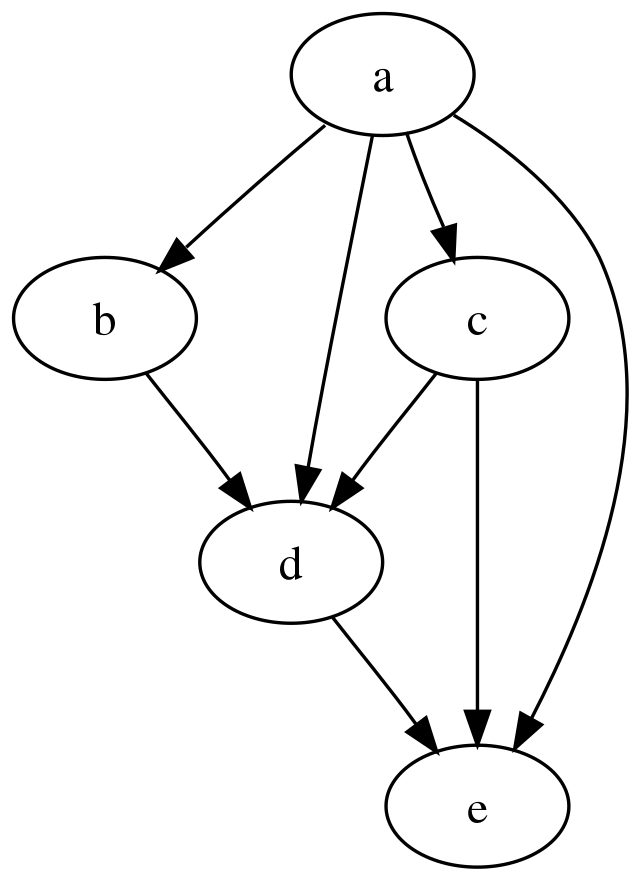
\includegraphics[width=6cm]{../ADG.png}
    \centering
    \label{fig:ADG}
\end{figure}

\textbf{NestJS} - To framework opiniowany i jako taki wymusza na użytkowniku stosowanie określonych wzorców.
Wykorzystuje progresywny JavaScript, jest zbudowany i w pełni obsługuje TypeScript oraz łączy elementy
programowania obiektowego, programowania funkcyjnego i reaktywnego programowania funkcyjnego.
W przypadku aplikacji internetowych Nest używa Express jako sterownika HTTP,
z opcjonalną konfiguracją Fastify. Zapewnia abstrakcję nad frameworkami,
ale jednocześnie udostępnia ich interfejsy API bezpośrednio programistom, zapewniając uncję wolności.
Jest dostarczany z dedykowanym interfejsem terminalowym, którego można użyć do uruchomienia projektu,
utworzenia nowego z zainstalowanymi wszystkimi zależnościami, generowania zasobów HTTP,
kontrolerów, usług, obiektów transferu danych i innych.

\subparagraph{Decyzja\\}

Zespół projektowy zdecydował się na wykorzystanie frameworka NestJS z wykorzystaniem
Fastify jako sterownik HTTP z uwagi na znaczną różnicę w wydajności względem sterownika Express.

Plusy oraz minusy takiej decyzji są następujące:

\begin{itemize}
    \item gotowa do wykorzystania architektura aplikacji;
    \item olbrzymia społeczność, od której można czerpać wiedzę na temat rozwiązań 
    oraz korzystać z gotowych rozwiązań popularnych problemów;
    \item mniejsza ilość kodu bazowego do napisania;
    \item prostsza separacja logiki biznesowej;
    \item ułatwione testowanie jednostkowe oraz integracyjne za pomocą wstrzykiwaniu
    zależności oraz wbudowanym narzędziom testowym;
    \item problematyczna implementacja rozwiązań nieprzewidzianych przez twórców
    frameworka;
    \item niski poziom kontroli nad cyklem życia żądań HTTP oraz samej architektury;
    \item komunikaty błędów mogą niewiele mówić programiście, co utrudnia proces debuggowania.
\end{itemize}

% Teoria - warum, co, gdzie, z kim?

% Narzędzia - decyzja, dlaczego?

\subsubsection{Aplikacja mobilna}

Teoria - warum, co, gdzie, z kim?

Narzędzia - decyzja, dlaczego?

\subsection{Założenia teoretyczne}

\subsection{Opis sytuacji faktycznej}

\subsection{Badania empiryczne/Inne}

\section{Zadania w projekcie}

\begin{longtable}{ | p{0.2\textwidth}| p{0.4\textwidth}| p{0.3\textwidth}| }
    \hline
    Cele szczegółowe projektu & Zadania w projekcie oraz termin rozpoczęcia i zakończenia realizacji zadania                                                                                    & Osoby zaangażowane w realizację zadania \\
    \hline
    \multirow[t]{9}{\linewidth}{Cel 1: Przygotowanie modeli uczenia maszynowego}
                              & \task{Zadanie 1: Zebranie danych kontekstowych}{1. Kacper Bylicki}{}{}{}
    \cline{2-3}
                              & \task{Zadanie 2: Przygotowanie danych treningowych}{1. Kacper Bylicki}{2. Jakub Barczewski}{3. Marek Gerszendorf}{}
    \cline{2-3}
                              & \task{Zadanie 3: Dobranie algorytmów uczenia maszynowego}{1. Kacper Bylicki}{}{}{}
    \cline{2-3}
                              & \task{Zadanie 4: Zaimplementowanie algorytmów uczenia maszynowego}{1. Kacper Bylicki}{2. Jakub Barczewski}{}{}
    \cline{2-3}
                              & \task{Zadanie 5: Przeprowadzenie testów i poprawek}{1. Kacper Bylicki}{}{}{}
    \hline
    \newpage
    \hline
    \multirow[t]{9}{\linewidth}{Cel 2: Przygotowanie aplikacji serwerowej sterującej algorytmami uczenia maszynowego}
                              & \task{Zadanie 1: Stworzenie diagramu architektury aplikacji}{1. Jakub Barczewski}{2. Kacper Bylicki}{}{}
    \cline{2-3}
                              & \task{Zadanie 2: Zaimplementowanie kanałów komunikacji między aplikacją serwerową, a aplikacją mobilną}{1. Jakub Barczewski}{}{}{}
    \cline{2-3}
                              & \task{Zadanie 3: Przeprowadzenie testów i poprawek}{1. Jakub Barczewski}{2. Kacper Bylicki}{3. Marek Gerszendorf}{}
    \cline{2-3}
                              & \task{Zadanie 4: Dokonanie optymalizacji aplikacji}{1. Jakub Barczewski}{}{}{}
    \hline
    \newpage
    \hline
    \multirow[t]{9}{\linewidth}{Cel 3: Przygotowanie aplikacji mobilnej}
                              & \task{Zadanie 1: Stworzenie diagramu architektury aplikacji}{1. Marek Gerszendorf}{}{}{}
    \cline{2-3}
                              & \task{Zadanie 2: Zaprojektowanie warstwy wizualnej na bazie diagramu}{1. Marek Gerszendorf}{2. Kacper Bylicki}{3. Jakub Barczewski}{}
    \cline{2-3}
                              & \task{Zadanie 3: Stworzenie prototypu aplikacji}{1. Marek Gerszendorf}{}{}{}
    \cline{2-3}
                              & \task{Zadanie 4: Zaimplementowanie kanałów komunikacji między aplikacją, a aplikacją serwerową}{1. Marek Gerszendorf}{2. Kacper Bylicki}{3. Jakub Barczewski}{}
    \cline{2-3}
                              & \task{Zadanie 5: Przeprowadzenie testów i poprawek}{1. Marek Gerszendorf}{}{}{}
    \hline
    \newpage
    \hline
    \multirow[t]{9}{\linewidth}{Cel 4: Przygotowanie dokumentacji technicznej projektu}
                              & \task{Zadanie 1: Stworzenie diagramu architektury projektu}{1. Marek Gerszendorf}{2. Kacper Bylicki}{3. Jakub Barczewski}{}
    \cline{2-3}
                              & \task{Zadanie 2: Rozrysowanie wzorca relacji w bazie danych (diagram ERD)}{1. Marek Gerszendorf}{2. Kacper Bylicki}{3. Jakub Barczewski}{}
    \cline{2-3}
                              & \task{Zadanie 3: Przygotowanie diagramu komunikacji aplikacji serwerowej oraz mobilnej}{1. Marek Gerszendorf}{2. Kacper Bylicki}{3. Jakub Barczewski}{}
    \cline{2-3}
                              & \task{Zadanie 4: Przygotowanie diagramu sekwencji do procesów aplikacji}{1. Marek Gerszendorf}{2. Kacper Bylicki}{3. Jakub Barczewski}{}
    \cline{2-3}
                              & \task{Zadanie 5: Stworzenie instrukcji instalacyjnej oraz developerskiej}{1. Marek Gerszendorf}{2. Kacper Bylicki}{3. Jakub Barczewski}{}
    \hline
\end{longtable}

\section{Efekty realizacji projektu}

\section{Użyteczność projektu}

\section{Autoewaluacja zespołu projektowego}

\section{Wykorzystane materiały i bibliografia związana z realizacją projektu}

Załączniki - mają być generowane automatycznie, do ogarnięcia :)

\end{document}
